\documentclass{paper}
\usepackage{graphicx}
\usepackage{url}
\usepackage[utf8]{inputenc}

\title{Research-Notes}
\author{Sameer Al Harbi}

\begin{document}
\part{Pandas}
\today
\begin{quote}
\url{https://pandas.pydata.org/docs/index.html}
\end{quote}
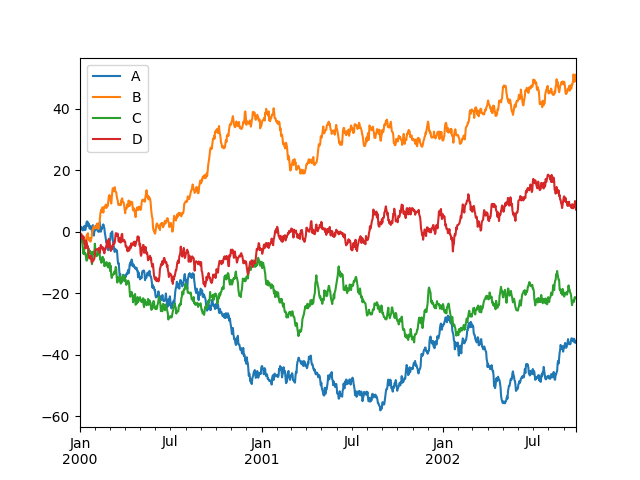
\includegraphics[width=180pt]{plot1.png}
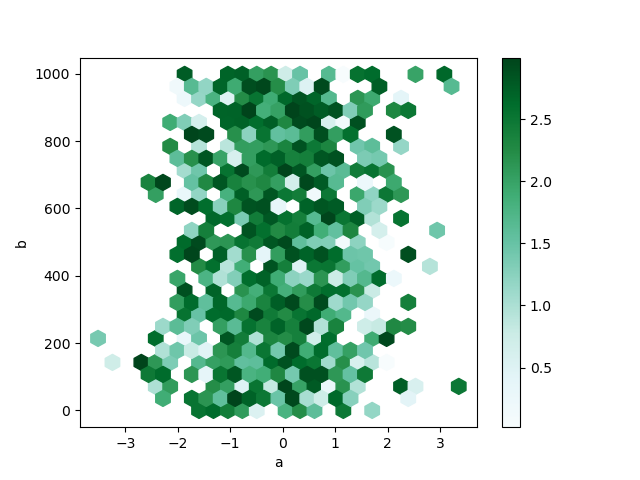
\includegraphics[width=180pt]{plot2.png}
\\
\\
\emp{Pandas is a python library that provides data structures and data analysis tools for data analysis and visualisation. Acting more as an API than a standalone program, Pandas supports multiple techniques that make calculating data and creating visuals easier- There is no implicit support for multidimensional data per say nor visuals but the tools provided probably can be used for it. 
}
\\
\\
\textbf{Key Points to takeaway from this}
\begin{enumerate}
    \item 2D data and graphs can be extended to numerous dimensions and viewed that way, many 2D plot over time or another dimension etc. Consider plotting 2D data then extending it
    \item consider how to render 2D views then extending them 
    \item consider what internal data analysis techniques can be run on the data as an extra
    
\end{enumerate}







\end{document}
